\chapter{Core concepts}\label{chapter:core_concepts}

After analyzing several \acrshort{orm}(s), we discovered significant differences among them, yet their core purpose remains identical. The primary objective is consistently retrieving data through queries and transforming database records into application objects based on a defined set of mapping rules.

The transformation is illustrated in Figure~\ref{fig:db_to_orm}. The database record is processed through an \acrshort{orm}, represented here as a black box containing predefined mapping rules, ultimately converting the data into a strongly typed C\# object.


\begin{figure}[h]
  \centering
  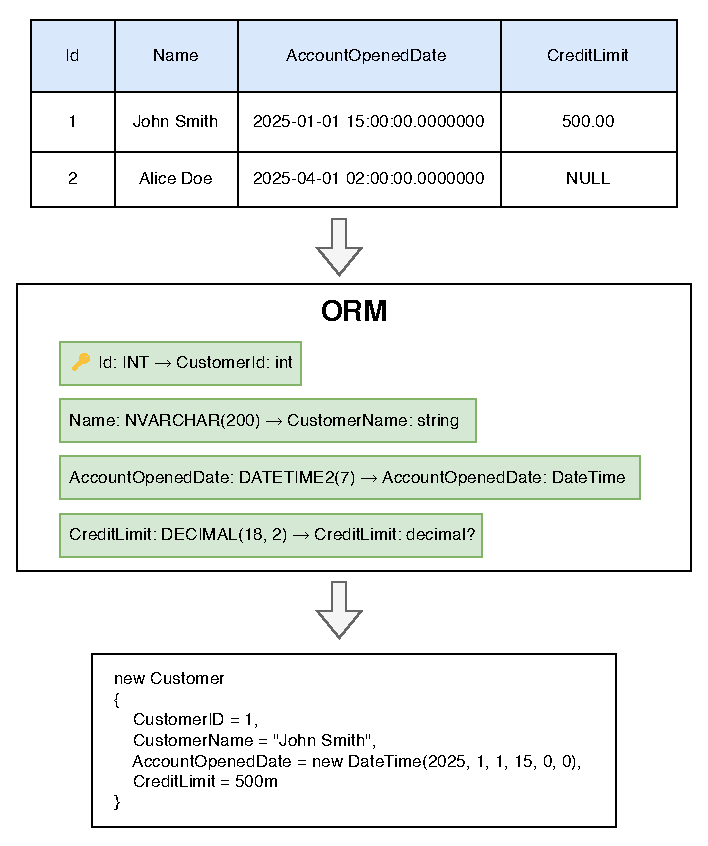
\includegraphics[scale=1.0]{thesis/img/thesis/02_orm_transformation.drawio.pdf}
  \caption{The process of converting database records to application objects using \acrshort{orm} with defined rules.}
  \label{fig:db_to_orm}
\end{figure}

Despite their common goals, significant performance differences across frameworks were observed during the evaluation in Section~\ref{sec:perf_eval}. For instance, query \hyperref[query:d3]{D3}, testing retrieval of one-to-many optional relationships, took over 2.5 seconds in \acrshort{ef} Core. In contrast, the same query executed with linq2db completed in just 91 milliseconds -- a performance improvement of more than twenty times. Clearly, performance differences among \acrshort{orm}s can be substantial.

Based on our observation, developers stick to using a single \acrshort{orm} per application, mainly to avoid complexity. However, combining multiple \acrshort{orm}s can be beneficial, particularly in performance-critical areas. For example, as noted in Section~\ref{sec:feat_dapper}, Dapper's creators explicitly suggest using it alongside another macro \acrshort{orm} to boost read performance where necessary. Nonetheless, employing multiple \acrshort{orm}s on the same database tables may introduce issues like data inconsistencies, particularly during write operations. Read operations do not modify the state of the database, and only read operations are explored in this work. Ensuring consistency remains a developer's responsibility when mixing \acrshort{orm}s.

Currently, converting queries from one \acrshort{orm} to another is challenging and typically requires manual work. Our approach will focus on automating this conversion process. We propose creating an abstraction that unifies entities, mappings, and queries into an intermediate representation, enabling efficient conversion between different \acrshort{orm} frameworks.

\section{Translation}\label{sec:core_translation}

In a .NET application, queries depend not only on the query statements themselves but also on entities and their respective mappings. While entities are always represented as C\# classes, mappings vary significantly. We have encountered mapping defined via attributes, fluent code syntax, and even \acrshort{xml} files. Despite these syntactical differences, the conceptual goal remains the same. The \acrshort{orm} has to be explicitly instructed how entities map to database tables, including data types, constraints, and relationships. To effectively automate query translation,common patterns across these diverse mapping strategies have to be identified.

Querying approaches differ similarly, primarily between raw \acrshort{sql} and strongly-typed \acrshort{linq} queries. RepoDB introduces a third variant, \textit{lambda functions}, but these functions can be viewed as a very limited subset of \acrshort{linq} and therefore are not considered separately. Regardless of the initial query method, all queries eventually get translated into \acrshort{sql} statements executed by the database. This observation makes \acrshort{sql} a logical basis for a unified abstraction layer.

By creating a common abstraction over entities, mappings, and queries, a unified intermediate representation can be achieved suitable for translation between different \acrshort{orm}(s). Implementing this intermediate representation significantly simplifies the translation task. Instead of requiring $N^2 - N$ direct conversions (each \acrshort{orm} to every other \acrshort{orm}, excluding self-conversions), the effort is reduced to just $2N$ conversions -- one into the intermediate representation and one out for each \acrshort{orm}. Additionally, not every conversion direction needs full support. For instance, translating from a deprecated \acrshort{orm} might be useful for migrations, but translating into it may be unnecessary.

Leveraging this approach, we will design and implement a tool that automates query conversion and facilitates easy performance comparisons across different \acrshort{orm} frameworks.

\section{User interaction}
To leverage the abstraction discussed earlier and showcase practical usage, we will create a conversion tool requiring user input consisting of three primary components, namely an \textbf{entity}, \textbf{mapping}, and a \textbf{query}. The tool will clearly define what inputs each supported \acrshort{orm} accepts, as not all \acrshort{orm}(s) utilize or even allow mapping. Users will have the option to manually specify the source \acrshort{orm} or rely on automatic detection by the tool.

During the parsing of the source entity, some information might be missing or not fully specified. If a database connection is supplied along with the source data, the tool could retrieve the necessary metadata (e.g., column types or constraints) directly from the database schema.

An illustrative scenario is depicted in Figure~\ref{fig:orm_to_abstract}. Here, the user selects Entity Framework Core as the source \acrshort{orm}. The interface will prompt for attributed entity or entities and a corresponding \acrshort{linq} query. Once the user provides these inputs and confirms the selection, our tool will internally parse them into the intermediate representation. Subsequently, this representation is used for translation into any other supported \acrshort{orm} chosen by the user. Missing entity mapping can be inferred by querying database metadata.

This interaction flow ensures a user-friendly workflow, while abstracting the complex translation process. The user does not need to know all the specific details of the target framework and what optimizations to perform. Additionally, this fast translation possibly allows for an automated performance comparison.

\begin{figure}[p]
  \centering
  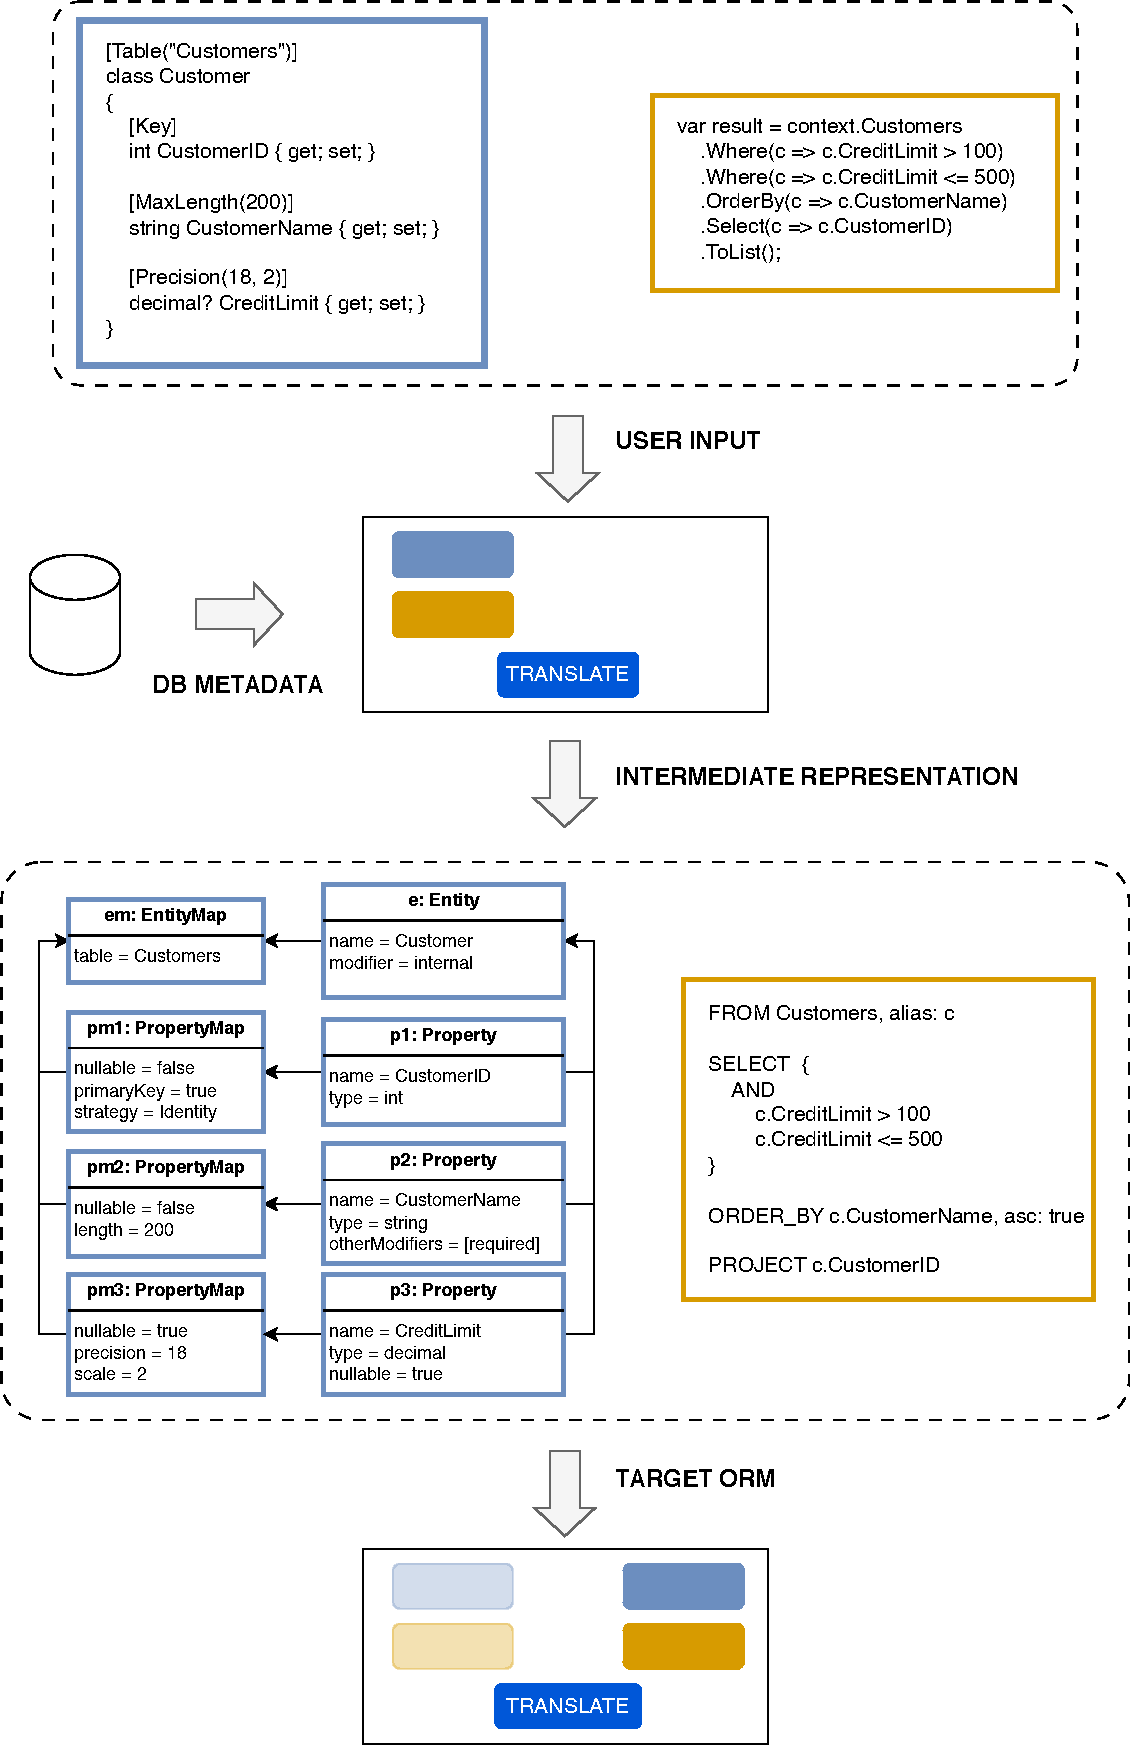
\includegraphics[width=\textwidth]{thesis/img/thesis/02_user_interaction.drawio.pdf}
  \caption{A demonstration of user interaction with the translation tool using an envisioned abstract representation.}
  \label{fig:orm_to_abstract}
\end{figure}

\section{Advisor}
Automating performance comparison between \acrshort{orm}s introduces both promising opportunities and also non-trivial challenges. We will refer to this tool as \emph{advisor}. At a high level, it would execute translated queries across target frameworks, measuring essential metrics such as runtime and memory usage. This automation would provide developers with insight into the performance implications of selecting one \acrshort{orm} over others. 

The advisor would rely on the intermediate representation to translate and run queries uniformly across supported \acrshort{orm}s in a controlled testing environment. Results would be evaluated against user-defined constraints. The constraints could be memory limits, runtime targets, or framework preferences. The user would be presented with one or more best options. This process would also support iterative tuning, allowing developers to refine queries or mappings and quickly observe performance implications.